\section{Multi-Cloud-Bibliotheken}
\label{sec:bibliotheken}

Ziel ist die Implementierung eines externen Broker-Services für den automatischen Betrieb mit mehreren Clouds. Da unabhängige Cloud-Provider keine einheitlichen APIs anbieten, stellt dieses Kapitel verschiedene Bibliotheken vor, um möglichst viel der zusätzlichen Komplexität zu verbergen, siehe \autoref{fig:multi-cloud-library}.

Ohne weitere Bibliotheken müsste für jede zu berücksichtigende Cloud das jeweilige SDK eingebunden werden. Auch Namensgebung, Architektur und Prozesse unterscheiden sich von Anbieter zu Anbieter.

\begin{figure}[ht]
%\begin{wrapfigure}{O}{0.3\textwidth}
	\centering
%	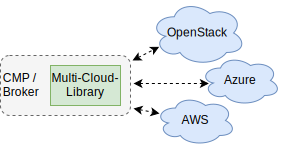
\includegraphics[width=0.48\textwidth]{images/multi-cloud-library.pdf}
		\def\svgwidth{0.48\textwidth}
		{\footnotesize \textsf{
		\includesvg{images/multi-cloud-library}}}
	\caption{Eingebette Bibliothek zur Multi-Cloud-Kommunikation.}	
	\label{fig:multi-cloud-library}
%\end{wrapfigure}
\end{figure}

Durch den Einsatz einer Drittbibliothek ergibt sich allerdings eine potenzielle Schwachstelle. Falls die Bibliothek fehlerhaft ist -- oder nicht weiter entwickelt wird -- gefährdet sie das gesamte Projekt. Historie und Zukunftschancen spielen bei der Auswahl eine zentrale Rolle. Im Optimalfall abstrahiert die Bibliothek alle zukünftigen Änderungen der Provider-SDKs. Ob und wie groß die Arbeitserleichterung ausfällt, prüft der Praxisteil.

Im Folgenden untersuchen wir die Eignung der populärsten Bibliotheken. Wichtigste Komponente ist dabei das Computing-Modul. Wünschenswert wäre auch Container-Unterstützung, um Images anbieterunabhängig bereitzustellen. Gestartete Anwendungskomponenten erfordern für die erste Erreichbarkeit oft Zugriff auf die DNS-Einstellungen der Cloud. Optional ist die Unterstützung von \emph{Content Delivery Networks}, Speicher- und Sicherungs-Diensten.

% https://tex.stackexchange.com/questions/341592/hyphenating-text-inside-tabularx
\begin{table*}\centering
	\begin{minipage}{\textwidth}
		\caption{Übersicht freier Multi-Cloud-Bibliotheken. Mit $*$ gekennzeichnete Eigenschaften sind experimentell. Aufgeführt sind nur die populärsten Cloud-Provider, die Bibliotheken können darüber hinaus weitere unterstützen. Ob eine Bibliothek weitere Informationen, wie aktuelle Preisinformationen und den Standort des Rechenzentrums abrufen kann, zeigt die Spalte \emph{Cost\,/\,Geo}.}
		\ra{1.3}
		\begin{tabularx}{\textwidth}{>{\centering}XXXr} \toprule
			Projekt & Cloud-Provider & Cloud-Services & Cost\,/\,Geo\\ \midrule
			Apache Libcloud (Python)\footnotemark & AWS, Azure, OpenStack, GCP, Docker & Compute, Container, DNS, Load Balancer, Storage, Backup & $x$\,/\,$x$\\
			Apache jclouds (Java)\footnotemark & AWS, Azure, Open\-Stack$*$, GCP, Docker & Compute, Container, Load Balancer$*$, Storage & $x$\,/\,$x$\\
			PkgCloud (Node.js)\footnotemark & AWS, Azure, OpenStack& Compute, Load Balancer, Storage$*$, DNS$*$ & --\,/\,--\\
			Libretto (Go)\footnotemark & AWS, Azure, OpenStack, GCP & Compute & --\,/\,--\\
			Fog (Ruby)\footnotemark & AWS, OpenStack, GCP & Compute, DNS, Storage & $x*$\,/\,--\\
			\bottomrule
		\end{tabularx}
		\label{tab:bibliotheken}
		\vspace{150pt}
		\footnotetext[1]{\url{https://libcloud.apache.org/}}
		\footnotetext[2]{\url{https://jclouds.apache.org/}}
		\footnotetext[3]{\url{https://github.com/pkgcloud/pkgcloud/}}
		\footnotetext[4]{\url{https://github.com/apcera/libretto/}}
		\footnotetext[5]{\url{http://fog.io/}}
	\end{minipage}  
\end{table*}

\autoref*{tab:bibliotheken} listet die untersuchten Bibliotheken mit unterstützten Cloud-Providern, Diensten und weiteren Funktionen. Letzteres sind Zugriff auf Preisinformationen des Anbieters und Standortinformationen der Rechenzentren. Zusätzlich sollten die Projekte kontinuierlich weiterentwickelt werden, eine aktive Entwicklergemeinschaft besitzen und gut dokumentiert sein. Alle sind quelloffen und unter einer freien Lizenz verfügbar.

\begin{description}
	
	\item[Apache jclouds] existiert schon seit 2009. Es unterstützt zumindest experimentell die wichtigsten Provider, aber nicht alle Dienste: DNS ist nicht vorhanden, Container-Unterstützung gibt es nur für Docker. Die Bibliothek ist gut getestet, dokumentiert, und mit zahlreichen Beispielen ausgestattet. Durch Java ist sie außerdem typsicher. 
	
	\emph{jclouds} ist außerdem Grundlage mehrerer Multi-Cloud-Projekte, z.\,B. von \emph{Apache brooklyn\footnote{\url{https://brooklyn.apache.org/}}}: Mithilfe von \emph{CAMP}-Plänen lassen sich Anwendungen über mehrere Clouds ausrollen.
	
	\item[Apache Libcloud] vereint eine Reihe von Vorteilen: Es unterstützt neben OpenStack -- als Referenz für Private-Cloud-Installationen -- sämtliche großen und kleinen Cloud-Provider mit allen Kernfunktionen. Besonders interessant ist die Container-Unterstützung für \emph{Docker}, \emph{Kubernetes}, \emph{Amazon ECS} und die \emph{Google Container Engine}. Entsprechend gepackte Anwendungen könnten in einer Vielzahl von Clouds ohne weitere Änderungen ausgeführt werden.
	
	\item[Fog] integriert die wichtigsten Anbieter und Dienste. Die Entwicklergemeinde rund um \emph{Fog} ist aktiv und die Bibliothek wird häufig eingesetzt. Besonders interessant sind die bereitgestellten Mocks, die als Platzhalter Tests neuer Integrationen erleichtern sollen. Zumindest für OpenStack wird Metering unterstützt, also die Abfrage bisher in Anspruch genommener Ressourcen. Eine einheitliche Namensgebung der verschiedenen Cloud-Produkte existiert nicht.
	
	\item[Libretto] beschränkt sich ausdrücklich auf die Compute-Funktionalität mithilfe virtueller Maschinen. Das zugehörige Projekt ist aktiv, kommt aufgrund der fehlenden Funktionalität aber nicht infrage.
	
	\item[PkgCloud] ist die einzige bekannte \emph{Node.js}-Bibliothek. Funktionsumfang und einheitliche Namensgebung der Cloud-Services sind überzeugend; leider wird die Bibliothek seit dem Verkauf des federführenden Unternehmens nicht mehr aktiv gepflegt. Bereits eingereichte Pull Requests werden nicht bearbeitet. Damit scheidet \emph{PkgCloud} für das Projekt aus.
	
\end{description}

\noindent Vielversprechend war außerdem das \emph{Apache-DeltaCloud}-Projekt: Aufbauend auf \emph{Ruby} stellt es nicht nur eine einheitliche API nach \emph{Cloud-Infrastructure-Management-Interface}-Standard\footnote{\url{https://www.dmtf.org/standards/cloud}} für die Kernfunktionen der wichtigsten Cloud-Provider, sondern auch zusätzliche Client-Bibliotheken und Mock-Funktionen. Aufgrund des plötzlichen Rückzugs von \emph{Red Hat} erfolgt seit 2013 allerdings keine Weiterentwicklung mehr \cite{androu:2013:deltacloud-red-hat-end}. Dieses Beispiel zeigt die Wichtigkeit nicht-funktionaler Betrachtungen bei der Auswahl einer Bibliothek. Auch Apache-Top-Level-Projekte haben nicht unbedingt eine sichere, vorhersagbare Zukunft.

Darüber hinaus existieren spezialisierte Bibliotheken wie \emph{SimpleCloud}\footnote{\url{https://framework.zend.com/manual/1.11/de/zend.cloud.html}} auf \emph{PHP}-Basis, das allerdings eine feste Komponente im \emph{Zend Framework} ist. Auch gibt es neue Entwicklungen wie \emph{CloudBridge}\footnote{\url{https://github.com/gvlproject/cloudbridge}} auf \emph{Python}-Basis. Besonderheit hier: Die Abstraktionsschicht nutzt die nativen SDKs der Cloud-Provider. \emph{CloudBridge} ist leider noch in einem frühen Entwicklungsstadium und als experimentell gekennzeichnet.

\emph{Libcloud} fasst die verschiedenen Cloud-Angebote nicht nur in gemeinsamen Namensräumen zusammen, sondern normalisiert auch Leistungsklassen. Python erleichtert außerdem den Einstieg und fügt sich in viele \emph{Python}-basierte Systemautomatisierungen ein. Diese Multi-Cloud-Bibliothek wird also im weiteren Verlauf der Arbeit erprobt.

%https://brooklyn.apache.org/learnmore/theory.html
% Apache Brooklyn hat eine eigene YAML-Service-Description-Spezifikation, ähnlich zu CAMP, der Clou Application Management API. Die Integration von TOSCA ist geplant, und in einer anderen Arbeit bereit umgesetzt: 
%Trans-Cloud: CAMP/TOSCA-based Bidimensional Cross-Cloud
% Keine SLAs, sondern nur Trigger-Action-Policies.
% Nutzt intern jclouds zur Provider-Anbindung.